\chapter{The Second Protocol - Covering Circuit Privacy}
\label{chap:renyiDivergence}

% **************************** Define Graphics Path **************************
\ifpdf
    \graphicspath{{Chapter4/Figs/Raster/}{Chapter4/Figs/PDF/}{Chapter4/Figs/}}
\else
    \graphicspath{{Chapter4/Figs/Vector/}{Chapter4/Figs/}}
\fi

\section{Introduction}
\label{sec:secProcIntro}
This chapter discusses Circuit Privacy, which is an important aspect of
Homomorphic Encryption, and how it affects the security of our first variant
of the protocol. We also describe a new technique being used to improve the
security proof of the protocol, to make sure that we can choose parameters small
enough for the system for practical reasons, but still preserve the security level. In
particular, we show how to use the infinity-order Renyi Divergence (RD) instead of
traditional Statistical Distance in the proof at security against a malicious client with exposed secret key, in order to significantly lower the initial noise bound parameter, which will result in a smaller moduli \(q\) for the ring \(R_{q}\) used by the
cryptosystem.

Circuit Privacy means that the ciphertext generated by a homomorphic operation
does not reveal anything about the circuit it evaluates, except its output
value. This property applies even to the party having generated the
keys.

Consider a ciphertext product result in a BV cryptosystem (section
\ref{sec:BVScheme}).
\[
  mult(c,c') = (\mathbf{c_0}\mathbf{c_0'}, \mathbf{c_0}\mathbf{c_1'} +
  \mathbf{c_1}\mathbf{c_0'}, \mathbf{c_1}\mathbf{c_1'})
\]
The noise term of this result ciphertext correlates to both $\mathbf{m}$ and
$\mathbf{m}'$. For example, given
$c = (\mathbf{b}\mathbf{r}_{1} + \mathbf{m}, -\mathbf{a}\mathbf{r}_{1})$ and $c' = (\mathbf{b}\mathbf{r}_{2} + \mathbf{m}', -\mathbf{a}\mathbf{r}_{2})$, the decryption result of $mult(c,c')$, which is its inner product with $(1,\mathbf{s}, \mathbf{s}')$, would include the noise term:
\[
t^{2}\mathbf{e}^{2}\mathbf{r}_{1}\mathbf{r}_{2} + t\mathbf{e}\mathbf{m}_{2}\mathbf{r}_{1} + t\mathbf{e}\mathbf{m}_{1}\mathbf{r}_{2} + \mathbf{m}_{1}\mathbf{m}_{2}
\]
In many
contexts, a leakage of this kind might be inconsequential for a genuine user
with a secret key, because s/he is supposed to know the key and decrypt the
message.  However, in many other contexts, especially in multi-factor
authentication scenarios, this is not the case. For instance, in our system, we
do not want the client to know the unmasked Hamming Distance value, so that an
attacker with a stolen device and a secret key cannot derive information about
the data stored in the server from the enrolment stage. We propose to mask this
data by homomorphically adding the ciphertext $Enc(HD, e)$ to $Enc(r, e')$ so as to
refresh the noise terms while masking the Hamming Distance at the same time ($e$ and $e'$ are the noises in the resulting ciphertext). The
question is how far from the original noise distribution we can move away
without compromising correctness, if this new security measure is applied.

Let $e$ denotes the noise in the original ciphertext $Enc(HD,e)$, for some fixed $e$, let $D_{1}$ be the probability distribution of the new shifted noise $e + e'$ of $Enc(HD + r, e + e')$ with respect to the choice of the mask noise $e'$ from Gaussian distribution with standard deviation $\sigma$. Let $D_{2}$ be the probability distribution of the unshifted noise $e'$. We observe that the
2 Gaussian distributions $D_{1}$ and $D_{2}$ are identical with the same standard deviation
$\sigma$ and different means. Let $r_0$ be the shift in the means of $D_1$ and $D_2$.
Our goal is to set up parameter $r_0$, such that $D_1$ and $D_2$ are computationally
indistinguishable while keeping other parameters of the cryptosystem within practical
performance
thresholds. Statistical Distance (SD) is normally used to measure the difference of distributions and can be shown to be
\[
SD(D_1, D_2) = \frac{1}{2}\sum_{x\in X}|D_1(x) - D_2(x)| \leq K\times \frac{r_0}
{\sigma}
\]
where $K$ is a constant. We quickly see that in order for $SD$ to be indistinguishable, ($SD < \epsilon \approx \frac{1}{2^\lambda}$, where $\lambda$ is
the security parameter), the standard deviation of the mask noise needs to be larger than $r_{0}$ by an exponential factor in $\lambda$, that is $\sigma \geq Kr_02^\lambda$.

In the work of \cite{bai2015improved}, the authors proposed Renyi Divergence (RD) as
an alternative to measure distributions' closeness and its applications to security proofs. $R_a(D_1\|D_2)$ of order $a$
between $D_1$ and $D_2$ is defined as the expected value of $(D_1(x)/D_2(x))^{a-1}$ over the randomness of $x$, sampled from $D_1$.
\[
R_a(D_1\|D_2) = \left( \sum_{x \in D_1}\frac{D_1(x)^a}{D_2(x)^{a-1}} \right)^
{\frac{1}{a-1}}
\]
Similar to SD, RD is useful in our context with its \textit{Probability Preservation} property (we refer readers to \cite{bai2015improved} for detailed formal
descriptions): Given $D_1$ and $D_2$ as described, for any event $E$, for instance, E may be the winning probability of an attacker in the distinguishing game, the probability of the event with respect to $D_2$ being bound by
\begin{align}
\label{eq:renyi}
D_2(E) \geq D_1(E)^{\frac{a}{a-1}}/RD_a(D_{1}\|D_2)
\end{align}
Particularly, if we look at the second order ($a = 2$) of RD as done in previous
works, we would have $ D_2(E) \geq D_1(E)^2/RD_2(D1\|D_2) $.  Provided that the
distribution functions on lattices of $D_1$ and $D_2$ are discrete Gaussian,
which is of the form
$\rho_\sigma(x) = \frac{1}{\sigma}e^{-\pi\frac{x^2} {\sigma^2}}$ ,
$RD_2(D_1\|D_2) = e^{2\pi \frac{r_0^2}{\sigma^2}} \approx e^{2\pi}$, when $r_0$
is much smaller than $\sigma$. This means that when switching from $D_1$ to $D_2$,
the success probability of $E$ will be at least the old probability to the power
of 2 divided by some constant. This squaring factor brings about a big trade-off: for
example, in our protocol, we would need to use $FAR = 2^{-20}$ in the
non-privacy biometric settings to get $FAR=2^{-10}$ into our scheme.

We aim at a solution to reduce this concrete security loss factor of the security proof. The idea is to look at $RD_\infty$
instead of at $RD_2$: from equation (\ref{eq:renyi}), we can infer that when $a$ is
large, $\frac{a}{a-1}$ approaches 1. However, for usual Gaussian distributions, the value of
$RD_\infty$ is also infinity (not a constant $e^{2\pi}$ like in $RD_2$ when
$a=2$). This is due to the ratios $\frac{D_1(x)}{D_2(x)}$, which become large when
sample is in the extreme tails of the distributions. Our idea is to
truncate the distribution when doing noise sampling: if we get a noise value
that is too close to the tail, we reject it and sample again. As a result, the $RD_{\infty}$ can be bounded by a finite amount. The
truncated distribution also scale up slightly (the small noises show
higher probability when sampling), but this does not have a high impact on security.


\section{Context and Related Work}
\label{sec:secProcPrevious}

\subsection{Definitions}
\label{sec:renyiDefinition}

% \subsubsection{Circuit Privacy}
% \label{sec:renyiCircuitPrivacy}

% To define Circuit Privacy, we view the operation of \(Evaluate\) (Section
% \ref{sec:defHomo}) as a protocol between a client who generates the keys and
% encrypts the input, and a server who evaluates some function on that input and
% returns the result to the client.

% \begin{definition}
%   [Circuit privacy.] A homomorphic encryption scheme E = (KeyGen,
%   Encrypt, Decrypt, Evaluate), correct for the circuit family C, is circuit
%   private for C, if there exists an efficient simulator Sim such that, for every
%   \(\tau \in \mathbb{N}, \pi \in C_{\tau},\) and plaintext bits \textbf{b} =
%   \((b_{1}, \dots, b_{t}) \in \{0,1\}^{t}\), one for every input bit of \(\pi\),
%   we have\\
%   $$Real_{\pi,\mathbf{b}}(\lambda) \approx Sim(1^{\lambda}, 1^{\tau},
%   \mathbf{b}, \pi(\mathbf{b}))$$ Where\\
%   \(Real_{\pi,\mathbf{b}}(\lambda) = \{(r,r',c): r, r' \randomsample \$, (sk,
%   pk) \gets KeyGen(1^{\lambda}, 1^{\tau}, r), c \gets Encrypt(pk, \mathbb{b},
%   r'), c' \gets Evaluate(pk, \pi, \mathbf{c})\}\)
% \end{definition}
% We note that the simulator \(Sim\) is given the output \(\pi(\mathbf{b})\) but
% not the description of the circuit \(\pi\) itself, and it needs to simulate the
% view that includes the randomness from key generation, encryption and
% ciphertext evaluation operations

% \subsubsection{Renyi Divergence}
% \label{sec:renyisubdefinition}
\begin{definition}
  [Renyi Divergence] Let \(Supp(D) = \{x: D(x) \neq 0\}\) denote the
  \textit{support} for a probability distribution \(D\). For any two discrete
  probability distributions \(P\) and \(Q\) such that
  \(Supp(P) \subseteq Supp(Q)\) and \(a \in (1, +\infty)\), the Renyi divergence
  of order a is defined by\\
  $$RD_{a} = \left(\sum_{x \in Supp(p)}\frac{P(x)^{a}}{Q(x)^{a-1}}\right)^{\frac{1}{a-1}}$$
\end{definition}
When \(a = 2\), the subscript is normally omitted, the Renyi divergence of
order \(+\infty\) is defined by
\(RD_{\infty} = max_{x \in Supp(P)}\frac{P(x)}{Q(x)}\). The definitions are
extended in the natural way to continuous distributions. The following
properties are considered analogues of those of Statistical Distance. Proofs can
be found in \cite{langlois2014gghlite}.
\begin{lemma}
  Let \(a \in [1, +\infty]\). Let \(P\) and \(Q\) denote distributions with
  \(Supp(P) \subseteq Supp(Q)\). Then the following properties hold:
  \begin{description}
  \item [Log. Positivity.] \(RD_{a}(P || Q) \geq RD_{a}(P||P) = 1\).
  \item[Data Processing Inequality]
    \(RD_{a}(P^{f} || Q^{f}) \leq RD_{a}(P || Q)\) for any function \(f\), where
    \(P^{f}\) and \(Q^{f}\) denote the distribution of \(f(y)\) induced by
    sampling \(y \randomsample P\) and \(y \randomsample Q\)
  \item[Multiplicative] Assume \(P\) and \(Q\) are two distributions of a pair
    of random variables \((Y_{1}, Y_{2})\). For \(i \in \{1,2\}\), let \(P_{i}\)
    and \(Q_{i}\) denote the marginal distribution of \(Y_{i}\) under \(P\) and
    \(Q\), and let \(P_{2|1}(\cdot | y_{1})\) and \(Q_{2|1}(\cdot | y_{1})\)
    denote the conditional distribution of \(Y_{2}\) given that
    \(Y_{1} = y_{1}\). Consequently:
    \begin{itemize}
    \item \(RD_{a}(P||Q) = RD_{a}(P_{1}||Q_{1}) \cdot RD_{a}(P_{2}||Q_{2}))\) if
    \(Y_{1}\) and \(Y_{2}\) are independent for \(a \in [1,\infty]\).
    \item
    \(RD_{a}(P||Q) \leq RD_{\infty}(P_{1} || Q_{1}) \cdot max_{y_{1} \in X}
    RD_{a}(P_{2|1}(\cdot | y_{1})||Q_{2|1}(\cdot | y_{1}))\)
    \end{itemize}
  \item[Probability Preservation] Let \(E \subseteq Supp(Q)\) be an arbitrary
    event. If \(a \in (1, +\infty)\), then
    \(Q(E) \geq P(E)^{\frac{a}{a-1}}/RD_{a}(P||Q)\) and
    \(Q(E) \geq P(E)/RD_{\infty}(P||Q)\)
  \item[Weak Triangle Inequality] Let \(P_{1}, P_{2}, P_{3}\) be three
    distributions with
    \(Supp(P_{1}) \subseteq Supp(P_{2}) \subseteq Supp(P_{3})\). Consequently:\\
    \(RD_{a}(P_{1}||P_{3}) \leq
    \begin{cases}
      RD_{a}(P_{1}||P_{2}) \cdot R_{\infty}(P_{2}||P_{3}),\\
      RD_{\infty}(P_{1}||P_{2})^{\frac{a}{a-1}} \cdot RD_{a}(P_{2}||P_{3})
      \text{if } a \in (1,+\infty)
    \end{cases}
\)
  \end{description}
\end{lemma}

\subsection{Related Work}
\label{sec:renyiRelatedWorks}
Ling et al. \cite{ling2017hardness} used RD as the framework for distinguishing
problems in the \textit{k}-LWE context, which is a variant of LWE in which the
adversary is given extra information in the distinguishing attack game. The
work of \cite{poppelmann2014enhanced27} used RD order 1 (Kullback-Leibler
divergence) to improve the communication size requirement of BLISS
\cite{ducas2013lattice11}. \cite{bai2015improved5} showed how generic RD can
be used as an alternative to the statistical distance in proofs for
lattice-based cryptography.  Bogdanov et al. \cite{bogdanov2016hardness4}
adapted the work of \cite{bai2015improved5} to the Learning With Rounding
problem. RD was used in \cite{libert2016signature} in the context of dynamic
group signatures and also in \cite{alkim2016post} to replace LWE noise
distribution by an easier to sample distribution.



\section{Renyi Divergence Analysis technique}
\label{sec:secProcRenyi}
% \subsection{Renyi Divergence and its application in noise masking}
% \label{sec:Renyi_original}

For the following analysis, let $D_1$ be a discrete Gaussian on $\mZ$ with
standard deviation parameter $\sigma$ shifted by the constant $r_0 \in \mZ$, while $D_2$
is a discrete Gaussian on $\mZ$ with deviation parameter $\sigma$ centered on zero,
i.e. $D_1 = D_{\mZ,\sigma} + r_0$ and $D_2 = D_{\mZ,\sigma}$, where
$$D_{\mZ,\sigma}(x) = \frac{e^{-\pi \cdot x^2/\sigma^2}}{\sum_{z \in \mZ} e^{-\pi \cdot
    z^2/\sigma^2}}, \text{ for } x \in \mZ$$
To allow us to use $RD_{\infty}$ we put
tail-cut variants $D_1^{(cut)}$ and $D_2^{(cut)}$ of $D_1$ and $D_2$ into play,
respectively with parameter $k$. The parameter $k$ defines where $D_1$ and $D_2$
are cut, for example, we can set $k=3$ to cut the distributions at 3 deviation
parameters from the mean. So, we let $D_{\mZ,\sigma}^{(cut)}$ denote
distribution $D_{\mZ,\sigma}$ tail-cut to the interval
$[-k \cdot \sigma, k \cdot \sigma]$ by rejection sampling.

We let $D_1^{(cut)} = D_{\mZ,\sigma}^{(cut)} + r_0$ and
$D_2^{(cut)} = D_{\mZ,\sigma}^{(cut)}$. Notice that the supports of
$D_1^{(cut)}$ and $D_2^{(cut)}$ are different, namely
$Supp(D_1^{(cut)}) = [-k\sigma+r_0,k\sigma+r_0]$ while
$Supp(D_2^{(cut)}) = [-k\sigma,k\sigma]$. We assume, without loss of generality,
that $r_0 > 0$. We would like to switch from distribution $D_1^{(cut)}$ to
$D_2^{(cut)}$, but unfortunately $R_\infty(\overline{D}_1^{(cut)}\|D_2^{(cut)})$
is not finite, since $Supp(D_1^{(cut)})$ is not a subset of
$Supp(D_2^{(cut)})$. To satisfy the latter condition, we first switch from
$D_1^{(cut)}$ to $\overline{D}_1^{(cut)}$ by further cutting (by rejection
sampling) the positive tail of $D_1^{(cut)}$ to ensure it does not go beyond the
$k \sigma$ upper bound on tail of $D_2^{(cut)}$, and use a (mild condition)
statistical distance step to lower bound $\overline{D}_1^{(cut)}(E)$. Then, in a
second step using
$Supp(\overline{D}_1^{(cut)})=[-k\sigma+r_0, k\sigma] \subseteq
[-k\sigma,k\sigma] = Supp(D_2^{(cut)})$, we derive a finite upper bound on
$R_\infty(\overline{D}_1^{(cut)}\|D_2^{(cut)})$ to lower bound
$D_2^{(cut)}(E)$. Details follow.

\begin{figure}[htbp!] 
  \centering
  \fbox{
    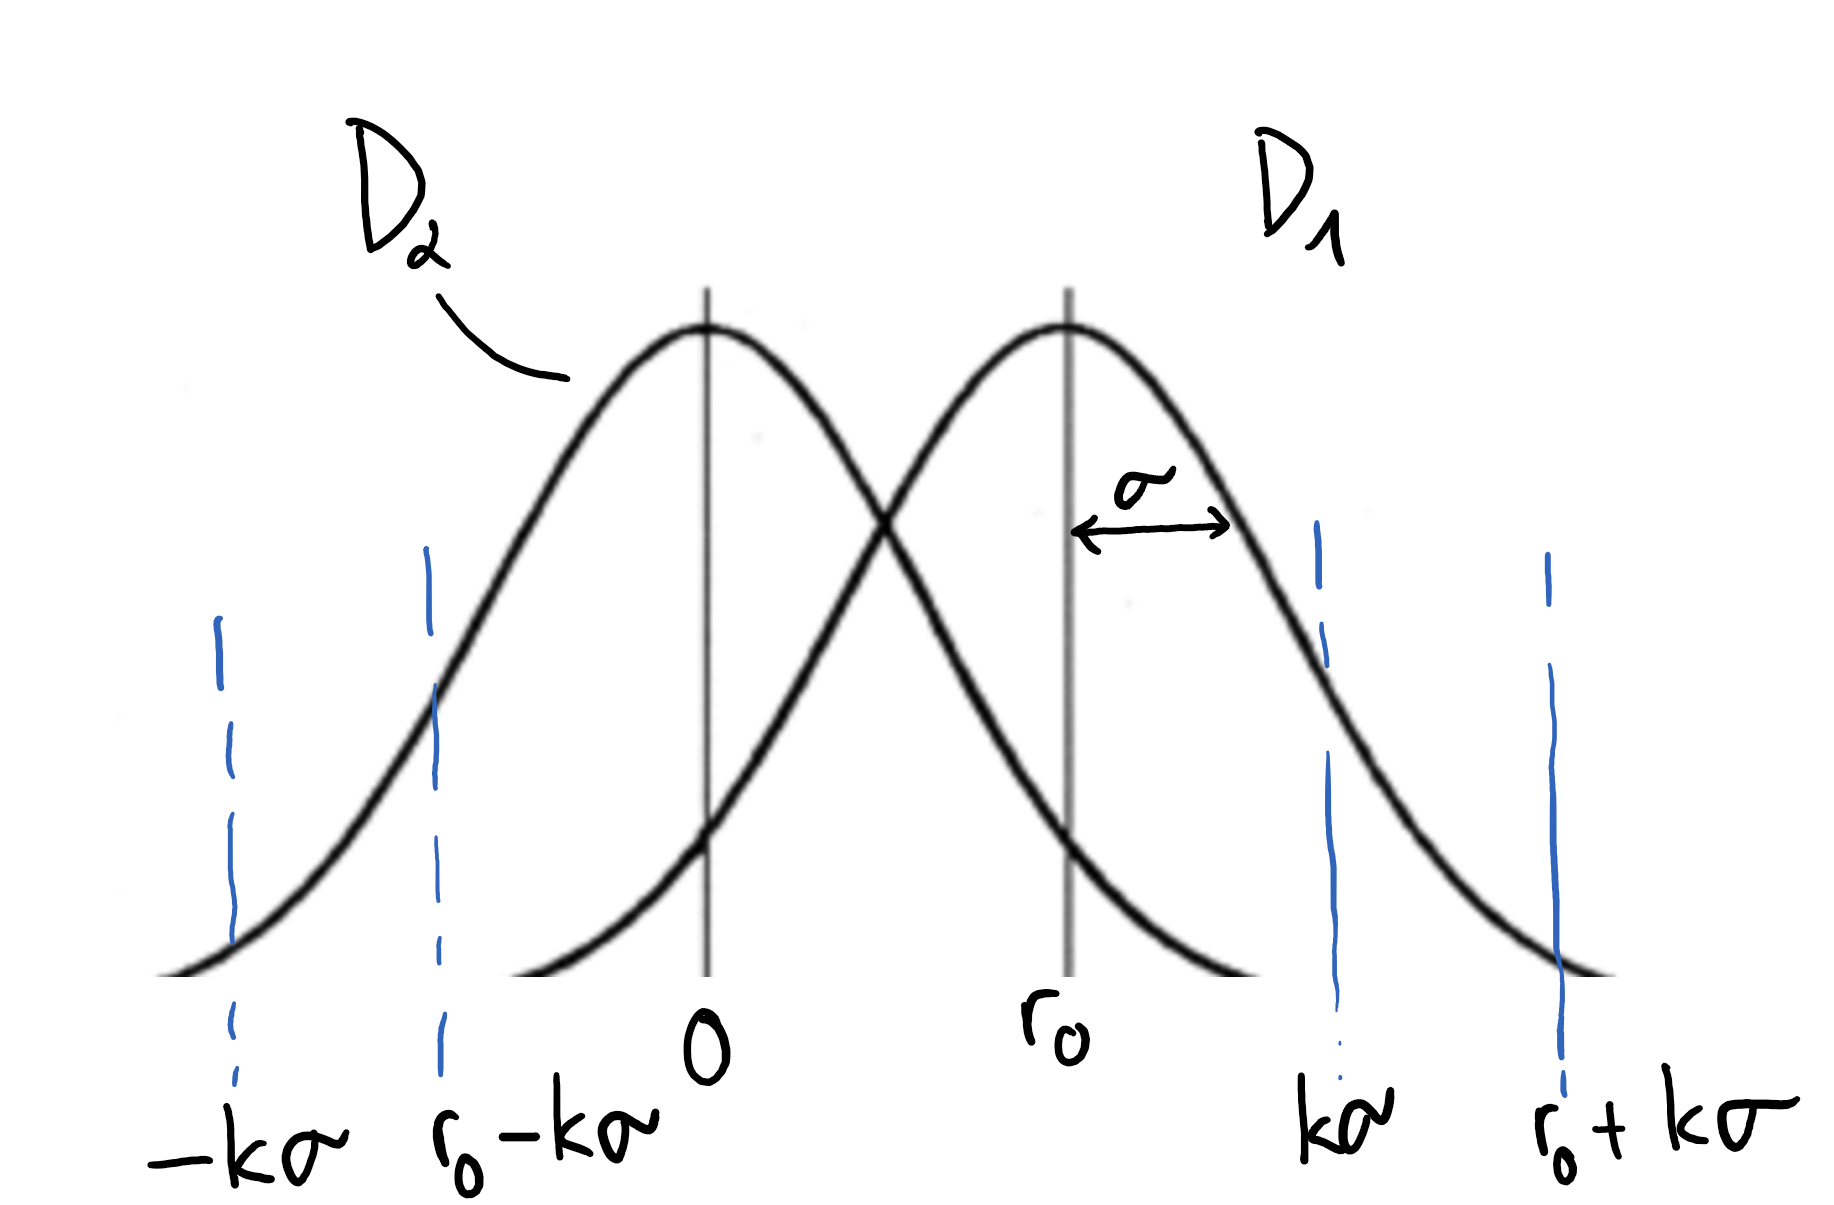
\includegraphics[scale=0.4]{Chapter5/rd}
    }
  \caption{Renyi Divergence tail cut}
  \label{fig:tailcut}
\end{figure}

\begin{sloppypar}
  \textbf{First SD Step.} Since $Supp(D_1^{(cut)})$ is transformed into
  $\overline{D}_1^{(cut)}$ by rejection and resampling if a sample of
  $Supp(D_1^{(cut)})$ falls in $(k\sigma,k\sigma+r_0]$, we have
  $$SD(D_1^{(cut)}, \overline{D}_1^{(cut)}) \leq
  D_1^{(cut)}((k\sigma,k\sigma+r_0]) = D_2^{(cut)}((k\sigma-r_0,k\sigma]) =
  D_{\mZ,\sigma}((k\sigma-r_0,k\sigma])/C_2$$, where
  $C_2 = D_{\mZ,\sigma}([-k\sigma,k\sigma])$. Consequently,
$$
\Delta \defeq \frac{D_{\mZ,\sigma}((k\sigma-r_0,k\sigma])}{C_2} = \frac{\sum_{z
    \in (k\sigma-r_0,k\sigma])} \e^{-\pi z^2/\sigma^2}}{\sum_{z \in
    [-k\sigma,k\sigma])} \e^{-\pi z^2/\sigma^2}}.
$$
For the numerator, we have the upper bound
\begin{align*}
  \sum_{z \in (k\sigma-r_0,k\sigma])} \e^{-\pi z^2/\sigma^2}
  &\leq \int^{\infty}_{k\sigma-r_0} \e^{-\pi z^2/\sigma^2} dz\\
  &\leq \sigma \cdot \e^{-\pi
    (k\sigma-r_0)^2/\sigma^2}
\end{align*}
The second inequality in the above bound is obtained by using the standard normal distribution tail upper bound
$$\int^{\infty}_{\gamma} \frac{1}{\sqrt{2\pi} \sigma} \cdot \e^{- z^2/\sigma^2}
dz \leq \e^{-\gamma^2/(2\sigma^2)}, \text{for }\gamma \geq 0 $$
For the denominator, we have the lower bound
\begin{align*}
  \sum_{z \in [-k\sigma,k\sigma]} \e^{-\pi z^2/\sigma^2}
  &\geq 2 \cdot \sum_{z \in [0,k\sigma])} \e^{-\pi z^2/\sigma^2}\\
  &\geq 2 \cdot (\int^{\infty}_{0} \e^{-\pi
    z^2/\sigma^2} dz - \int^{\infty}_{k\sigma} \e^{-\pi z^2/\sigma^2} dz)\\
  &\geq \sigma \cdot (1 - 2 \cdot \e^{-\pi (k\sigma-r_0)^2/\sigma^2})
\end{align*}
Therefore,
$SD(D_1^{(cut)}, \overline{D}_1^{(cut)}) \leq \Delta \leq \delta' / (1-2\delta')
\leq 2\delta'$ if $\delta' \leq 1/4$, where
$\delta' = \e^{-\pi (k\sigma-r_0)^2/\sigma^2}$. Defining $\delta = 2\delta'$, makes $\Delta \leq \delta$ if $\delta \leq 1/2$ and the conditions
$r_0 \leq \sigma$ and $k \geq 1 + \sqrt{1/\pi \cdot \ln(2/\delta)}$
hold. Therefore, by the probability preservation property, for any event $E$, 
$\overline{D}_1^{(cut)}(E) \geq D_1^{(cut)}(E) - \delta$ holds.
\end{sloppypar}
% with probability $D_1^{(cut)}(E)$ \geq \varepsilon$, we have can take $\delta
% = \var{\epsilon This tells us how to set the tail cut parameter $k$.

\textbf{Second RD step.} The desired RD of order $\infty$ is defined by
\[
  R_\infty(\overline{D}_1^{(cut)}\|D_2^{(cut)})) = \max_{x \in
    [-k\sigma+r_0,k\sigma]} \frac{\overline{D}_1^{(cut)}} {D_2^{(cut)}(x)}.
\]
Observe that, for each $x \in [-k\sigma+r_0,k\sigma]$, we have
$\overline{D}_1^{(cut)}(x) = C \cdot D_1^{(cut)}(x)$, where the normalization
constant
\begin{align*}
  C &= \frac{1}{1-D_1^{(cut)}((k\sigma,k\sigma+r_0])}\\
    &= \frac{1}{1-D_2^{(cut)}((k\sigma-r_0,k\sigma])}\\
    &= \frac{1}{1-\Delta}
\end{align*}
Where $\Delta$ is defined and upper bounded by $\delta$ above, under the assumed
conditions on $k$ and $\delta$. Since the $D_1^{(cut)}(x)$ and $D_2^{(cut)}(x)$
are shifts of each other, they have the same rejection sampling normalization
constant with respect to $D_1$ (resp. $D_2$). Therefore,
$D_1^{(cut)}(x)/D_2^{(cut)}(x)=D_1(x)/D_2(x)$ for each $x$ in the support of
both $D_1^{(cut)}$ and $D_2^{(cut)}$, and thus
% $D_1(x)$ and $D_2(x)$ divided by some constant factor $C_1$ and $C_2$ (to keep
% the cumulative probability area to be 1) . In our context, as $D_1(x)$ and
% $D_2(x)$ are the same distributions with different means, so $C_1 = C_2$.
\begin{align*}
  R_\infty(\overline{D}_1^{(cut)}\|D_2^{(cut)}) &\leq \frac{1}{1-\delta} \cdot \max_{x \in [-k\sigma+r_0,k\sigma]} \frac{D_1(x)}
                                                  {D_2(x)}\\
                                                &= \max_{x \in [-k\sigma,k\sigma]}\frac{e^{\frac{-\pi(x-r_0)^2}{\sigma^2}}}{e^{-\pi\frac{x^2}{\sigma^2}}}
  \\
                                                &= e^{\pi \cdot r_0^2/\sigma^2} \cdot \max_{x \in [-k\sigma+r_0,k\sigma]}e^{\frac{2\pi r_0}
                                                  {\sigma^2}x}
\end{align*}
This is an exponential function yielding its max value at $x = k\sigma$:
$$
R_\infty(\overline{D}_1^{(cut)}\|D_2^{(cut)}) = e^{1/(1-\delta)} \cdot e^{\pi
  \cdot r_0^2/\sigma^2 + 2\pi k \cdot r_0/\sigma}.
$$
Since $0<\delta \leq 1/2$, the first factor above is
$\leq 1+2\delta \leq e^{2\delta}$. Also, a simple computation shows that the
second factor is less than $e$ if the condition $\sigma/r_0 \geq 4 \pi \cdot k$ is
satisfied using $k \geq 1$. We conclude, under the assumed parameter conditions,
that
$R_\infty(\overline{D}_1^{(cut)}\|D_2^{(cut)})) \leq e^{1+2\delta} = c'(\delta)$
is constant for a constant $\delta>0$, so that, by the RD probability preservation
property,
\begin{align*}
  D_2^{(cut)}(E) &\geq \frac{1}{c(\delta)} \cdot \overline{D}_1^{(cut)}(E)\\
                 &\geq \frac{1}{c(\delta)} \cdot (D_1^{(cut)}(E) - \delta)
\end{align*}
Note that if $D_1^{(cut)}(E)=\varepsilon$, then, by choosing
$\delta = \varepsilon/2$, we get
$D_2^{(cut)}(E) \geq \frac{1}{2c(\delta)} \cdot \varepsilon$, and we only need
$k \geq 1 + \sqrt{1/\pi \cdot \ln(2/\delta)}$ and $\sigma/r_0$ logarithmic in
$1/\delta$, much smaller than $\sigma/r_0$ linear in $1/\delta$, which we would
need if we were to use the `SD only' analysis approach.

The above discussion immediately generalizes from the one-dimensional case of
discrete Gaussian samples over $\mZ$ to the $m$-dimensional case of discrete
Gaussian samples over $\mZ^m$, due to the independence of the $m$
coordinates. The only change to the above argument is that the statistical
distance in the `SD step' can multiply by at most a factor $m$, whereas the RD
in the `RD step' above gets raised to the $m$'th power, where we replace $r_0$
by $\|\vec{r}_0\|_{\infty}$. We compensate it by replacing the bound
$\delta$ on $\Delta$ in the above analysis by the bound $\delta/m$. We have
therefore proved the following result used in our impersonation security proof,
which improves upon the $R_2$-based analogue result for shifted Gaussians stated
in~\cite{langlois2014gghlite}.

% \keq Note that when $r_0$ is much smaller than $\sigma$, the first term
% $e^{\frac{\pi r_0^2}{\sigma^2}} \approx 1$. However, if $r_0$ is too small
% compared to $\sigma$, then the second term is at most $e^{2k\pi}$, which is
% also very large in the relation of equation (\ref{eq:renyi}). Or, we can also
% choose parameters such as $k = 3$ and $\frac{r_0}{\sigma} = \frac{1}{6}$, then
% the trade-off factor becomes much smaller, $e^{\pi}$. In conclusion, by
% applying infinity order RD to measure the truncated distributions closeness,
% we might obtain better parameters ($\sigma \geq 6r_0$, for example, compared
% to $\sigma \geq Kr_02^\lambda$ in SD approach) while providing
% \textit{Probability Preservation}, or security against distinguishing
% adversaries.

\begin{lemma} \label{le:Renyi} For integer $m \geq 1$, real
  $\sigma>0$,$k \geq 1$, real $0<\delta \leq 1/2$ and vector
  $\vec{r}_0 \in \mZ^m$, let
  $D_1^{(cut)} = D_{\mZ^m,\sigma}^{(cut)} + \vec{r}_0$ and
  $D_2^{(cut)} = D_{\mZ^m,\sigma}^{(cut)}$ be relatively shifted tail-cut
  discrete Gaussian distributions, where $D_{\mZ^m,\sigma}^{(cut)}$ is the
  discrete Gaussian $D_{\mZ^m,\sigma}$ with its tails cut to the support
  $[-k\sigma,k\sigma]^m$ by rejection sampling. If the conditions
  $k \geq 1 + \sqrt{1/\pi \cdot \ln(2m/\delta)}$ and
  $\sigma/\|\vec{r}_0\|_{\infty} \geq 4 \pi \cdot k \cdot m$ hold, then, for any
  event $E$ defined over the support of $D_1^{(cut)}$, it is the case that
$$
D_2^{(cut)}(E) \geq \frac{1}{2e^{1+2\delta}} \cdot \left(D_1^{(cut)}(E) - \delta\right).
$$
\end{lemma}

\section{The authentication protocol}
\label{sec:our_protocol}
The application to our protocol mainly happens in the step of masking the value of $HD$. In addition to masking $HD$ with some value $r$, we also need to mask the correlated noise used in the encryption process. The rest of the protocol steps are identical to Section \ref{sec:protocol1specs}.
\begin{description}
\item[Setup.] $\user$ and $\server$ initialize the parameters, taking into account the following categories:
  \begin{description}
  \item[Biometric Authentication System Parameters.] These parameters are
    standard ones used by non privacy preserving biometric authentication
    systems:
    \begin{itemize}
    \item False Acceptance Rate (FAR) and False Rejection Rate (FRR)
    \item $a$: The maximum number of incorrect authentication attempts allowed
      by $\server$.
    \item $\tau$: Threshold to compare the Hamming Distance to decide the
      authentication result.
      % \item $B$: An integer defines the base of the HD in a
      %   decomposition operation.
    \item \(n'\): The bit-length of the encoded biometric data.
    \end{itemize}
  \item[Ring-LWE based techniques parameters.] These parameters are used in the
    lattice-based cryptosystem which provides client privacy against long term
    quantum attacks.
    \begin{itemize}
    \item $\lambda$: General security parameter of the cryptosystem (the
      adversary's winning chance in the CPA security game is \(1/2^{\lambda}\))
    \item $n$: Integer $n$ defining the plaintext and ciphertext rings. This
      will be refered to as the degree of the polynomial objects or dimension of
      the underlying lattice during correctness and security proofs.
    \item $t$: Integer $t$ defining the plaintext space ring
      $R_t = \mathbb{Z}_t[x]/x^n+1$.
    \item $q$: Integer $q$ defining the ciphertext space ring
      $R_q = \mathbb{Z}_q[x]/x^n+1$
    \item $\chi_{\alpha q}$: A distribution used to sample noises for LWE-based
      techniques.  Typically, $\chi$ is a Gaussian distribution with standard
      deviation $\alpha q$.
    \item \(\delta\): Renyi Divergence parameter for the security of noise
      masking.
    \end{itemize}
  \item[Keygen.] Keys are generated for $\user$:
    \begin{itemize}
    \item Secret key: $\mathbf{s} \randomsample \chi_{\alpha q}^n$,
      \(sk = (1, \mathbf{s, s^{2}, ...})\)
    \item Public key: $pk = \mathbf{(p_0,p_1)}$, with
      $\mathbf{p_1} \randomsample R_q$ and
      $\mathbf{p_0} = -\mathbf{p_1s} - t\mathbf{e}$, with
      $\mathbf{e} \randomsample \chi_{\alpha q}^n$.
    \end{itemize}
  \end{description}
\item [Enrolment.] $\user$ extracts the biometric template $\mathbf{x}$, the bit
  string $\mathbf{x}$ being represented as a ring element of ${R}_t$.  The
  encryption is done by $\enc{\mathbf{x}} = (\mathbf{c_0},\mathbf{c_1})$ and
  sent to $\server$.
\item [Authentication.] The following steps are required:
  \begin{enumerate}
  \item $\user$ extracts his biometric features again $\mathbf{y}$ to use them
    as the query. $\user$ sends $\enc{\mathbf{y}} = (\mathbf{c_0', c_1'})$ to
    $\server$.
  \item ZKP for the first relation: $\user$ has to prove that $\enc{\mathbf{y}}$
    is a valid encryption, that is, it encrypts a bit string under the BV
    cryptosystem using the corresponding secret key. This is done by module
    \textbf{SternBV(A, y, x)} described in Sect. \ref{sec:Stern-basedZKP}, where
    $\mathbf{A} = \begin{bmatrix} c_{y0}, t, 0, 1\\p_{y0}, 0, t, 0
    \end{bmatrix}$, \(\mathbf{X} = [\vec{s},\tilde{e_{y}},\vec{e_{0}},y]^T\) and \(\mathbf{Y
    = [c_{y1},p_{y1}]}^{T}\).

\item HD Computation: $\server$ computes $\enc{HD_{\mathbf{x,y}}}$ using
  procedure \ref{sub:ciphertext_packing}. We note that the noise term
  $\mathbf{e_{HD}}$ of $\enc{\mathbf{HD,e_{HD}}}$ can leak information about
  $\mathbf{x}$ when $\mathbf{HD}$ is decrypted. Therefore, an extra step is
  needed to secure the operation.
  \begin{itemize}
  \item Sample $\mathbf{e_{r}} \randomsample \chi_{r}^n$ such that
    $\norminf{\mathbf{e_r}}$ is big enough compared to
    $\norminf{\mathbf{e_{HD}}}$.(Section \ref{sec:secProcRenyi})
  \item Compute $\enc{\mathbf{r,e_r}}$ and carry out an homomorphic addition
    operation to mask both the values of $\mathbf{HD}$ and the noise
    $\mathbf{e_{HD}}$:
    $\enc{\mathbf{HD', e'_{HD}}} = \enc{\mathbf{HD, e_{HD}}} +
    \enc{\mathbf{r,e_r}}$
    \end{itemize}
    The result $\enc{\mathbf{HD'}}$ is then sent to $\user$.
  \item \(\user\) decrypts $\enc{\mathbf{HD'}}$ and derives the actual value
    ${HD'}$ from the first coefficient of the plaintext:
    \( dec\enc{\mathbf{HD'}} = HD' + r_1 + r_2 + \dots + r_{n-1} \). \(\user\)
    sends \(HD'\) to \(\server\).
  \item \(\user\) proves that it does the decryption honestly, this is done
    similarly to step 2.
  \item \(\server\) unmasks \(HD'\) and outputs the authentication result
    \(HD \stackrel{?}{<} \tau\)
  \end{enumerate}

\end{description}

\subsection{Security Analysis}
\label{sec:protocol2SecurityProof}
\begin{theorem}[Server side security]
  \label{theo:serverprotocol2}
  Under the IND-CPA security of BV cryptosystems, and the zero-knowledge property of the Stern protocol, the proposed
  scheme satisfies (Honest But Curious) Server Privacy Security.
\end{theorem}
\begin{theorem}[Client side security]
  \label{theo:clientprotocol2}
  Under the IND-CPA security of BV cryptosystem and the soundness property of
  the underlying Stern protocol, the proposed scheme satisfies Impersonation and
  Multifactor Security. Concretely, for $\delta>0$, the protocol is
  $(q,c)$-secure against impersonation with $c \leq c(\delta) + 3 \cdot c_1$,
  assuming the underlying non-private biometric protocol has impersonation
  probability $\varepsilon_{bio}$ and the underlying Stern ZK protocols have
  knowledge error $\eps_{ZK1},\eps_{ZK2}$ such that
  $q(\varepsilon_{ZK1}+\varepsilon_{ZK2}) + \delta \leq c_1 \cdot
  \varepsilon_{bio}$, $c(\delta) = 2 e^{1+2\delta}$, and the condition
  $\sigma/r_0 \geq 4 \pi k n q$ holds, for
  $k = 1 + \sqrt{1/\pi \ln(2nq/\delta)}$ and $r_0$ as an upper bound on the size
  of the noise in $\enc{\mathbf{HD}}$.
\end{theorem}

The proof for Theorem \ref{theo:serverprotocol2} can be obtained as described in
Section \ref{sec:securityPro1}. For Theorem \ref{theo:clientprotocol2}, there is
a minor game change in the client impersonation model after game 4. We briefly
recall the game sequence; the detailed
diagrams of the changes in consecutive games can be found in Section
\ref{sec:securityPro1}.

\textit{Game 0} (Figure \ref{fig:game0protocol1client}). Game 0 is the original
impersonation game for type I attack.
\begin{description}
\item [Setup.] $\challenger$ intiates $D_k \randomsample D_{bio}$ and
  $X_k \randomsample D_k$. $\challenger$ sets up $(sk_k, pk_k)$ and launches
  $Enrol(k, X_k)$ to get $(sk_k, \enc{\mathbf{X}_{k}} =(pk_k, \mathbf{X}_{k}))$.
  $\attacker$ submits a type 1 attack query and receives $sk_k$ from
  $\challenger$.
\item [Query.] $\attacker$ runs $q$ authentication sessions. In each session
  $j = 1, \dots, q$, $\attacker$ can choose $\mathbf{Y}_{i} \gets \{0,1\}^{n}$
  and sends $\enc{\mathbf{Y}_{i}}$. $\attacker$ and $\challenger$ run
  $\mathbf{ZKPoPK1}$. $\challenger$ evaluates $\enc{\mathbf{HD}_{k}}$ then
  computes $\enc{\mathbf{HD'}_{k}}$. The resulting ciphertext is sent to
  $\attacker$, $\attacker$ decrypts $\enc{\mathbf{HD'}_{k}}$ and sends back the
  plaintext value of $HD'_{i}$. $\attacker$ and $\challenger$ run
  $\mathbf{ZKPoPK2}()$. $\challenger$ computes $HD = HD' - r$, compares the result to $\tau$, and sends back the authentication result $\mathbf{Accept}$ or \textbf{Reject} to $\attacker$ .
\item [Guess.] At the end of the game, $\adv$ outputs $\mathbf{Y'}$.
\end{description}

Next, we discuss following games, the plan being to proceed towards the final
game, where everything related to $X_k$ that $\attacker$ receives can be simulated
without any knowledge about $X_k$ (the only known information about $X_k$ is the
function $Verify(X_k, Y)$). Let $res_i = Verify(X_k, Y_{i})$ and $S_j$ be
the event in the game $j$ such that $res_j = Accept$.\\

In the \textit{Game 1} and \textit{Game 2}, the real ZKPs are replaced by the
\textbf{ZKPSimulator}, by the end of \textit{Game 2}, if in any authentication
attempt $i$, none of the 2 games have been aborted, then, by the correctness
property of ZKP, the server's output is equal to the output of
$Verify(X_k, Y_{i})$. In other words, we have shown what we could get by just
querying the oracle $Verify()$. Next, we want to simulate everything related to
$X_k$ the attacker
can see using just that oracle.\\

\textit{Game 3.} At the end of \textit{Game 2}, $\challenger$ has the bit
$b = Verify(Y^{(i)},X_k)$. In this game, we can change $res_{i}$ from
$compare(HD_{i},\tau)$ to $Verify(X_{k},Y_{i})$. By doing this change,
$\attacker$ still sees the same result, so the probability of winning of
$\attacker$ in this game is the same as in \textit{Game 2}: $\prob{S_{3}} = \prob{S_{2}}$
\\

\textit{Game 4.} In this game, we change the way $\challenger$ computes
$\enc{\mathbf{HD'}_{i}}$: In the orignal game 0, $r$ was added to mask the value
of $HD$. We want to prevent this $r$ from being used anywhere in the game, so we
replace $\enc{r}$ by $\enc{0}$. This change does not affect $\attacker$'s
success probability: $r$ only affects the plaintext inside $\enc{\mathbf{HD'}}$,
since we do not use this plaintext anymore (it has been replaced in \textit{Game
  3}), this
change therefore does not affect what the attacker sees. Again, $Pr[S_4] = Pr[S_3] = Pr[S_2]$.\\

% After we finish \textit{Game 4}, we can see that all the messages the attacker
% sees, can be simulated using only the verified bit $b = Verify(Y^{(i)},
% X_k)$. We now have an attacker $A'$ against the biometric impersonation with
% advantage:
% \[
% \varepsilon_{bio} = Adv(A') = Pr[S_4] \geq (\varepsilon_{imp} - q(\varepsilon_{ZK1}+\varepsilon_{ZK2})) ,
% \]
% which results in the claimed bound.

\textit{Game 5.} We modify the way $\enc{\mathbf{HD}}$ is computed in this game. Instead
of calculating
$\enc{\mathbf{HD'}_{i}} = \enc{\mathbf{HD}_{i}} + \enc{\mathbf{r}_{i}}$, the
challenger chooses a random $HD' \randomsample \mathbb{Z}_p$ and encrypts it
with the noise used before. In this game, the plaintext has changed from being
$r + HD$ to a uniform $HD' \in \mathbb{Z}_p$.  Since $r$ is also uniform in
$\mathbb{Z}_p$, the attacker is confronted with a uniform
plaintext in both cases. Therefore, $Pr[S_5] = Pr[S_4]$.
\\\\
\textit{Game 6.} Finally, we set $\enc{\mathbf{HD'}_{i}} = Enc(HD'_{i}, e_{HD'_{i}})$ for
$e_{HD'} \randomsample \chi_{mask}$ instead of $e_{HD} + e_{r}$. We replace
the sum of the Gaussian noise with a random noise. In Section \ref{sec:secProcRenyi},
we showed that $Pr[S_6] \geq \frac{1}{c(\delta)}(Pr[S_5]-q \cdot \delta)$, where
$c(\delta) = RD(e_{HD} + e_{r}, e_{HD}) \leq 2 \cdot e^{1+2\delta}$ by
Lemma~\ref{le:Renyi} and by our assumption on the parameter's values. After we
finish \textit{Game 6}, we notice that all the messages available to the
attacker can be simulated with only the verified bit $b = Verify(Y^{(i)},
X_k)$. We now have an attacker $A'$ against the biometric impersonation with
advantage:
\[
\varepsilon_{bio} = Adv(A') = Pr[S_6] \geq \frac{1}{c(\delta)}(\varepsilon_{imp} - q(\varepsilon_{ZK1}+\varepsilon_{ZK2} +) + \delta),
\]
which gives the claimed bound $\varepsilon_{imp} \leq c(\delta) \cdot \varepsilon_{bio} + q \cdot (\varepsilon_{ZK1}+\varepsilon_{ZK2}) + \delta \leq (c(\delta)+c_1) \cdot \varepsilon_{bio}$ if $q(\varepsilon_{ZK1}+\varepsilon_{ZK2}) + \delta \leq c_1 \cdot \varepsilon_{bio}$.

\subsection{Security Proof for Type II Impersionation attack}
\label{append:ProofsTypeII}
This proof can also be provided using a sequence of games between the challenger
$\challenger$ and the adversary $\attacker$. We present a sequence of games as
well as the relations among them to demonstrate the type II security model
proof. The idea is that in this type of attack, $sk_k$ is not used to compute
the view of $\attacker$.  On the other hand, the soundess of the zero-knowledge
proof of knowledge $\mathbf{ZKPoPK}$ implies the existence of an efficient
witness extractor algorithm, capable of extracting the witness (i.e. the
secret key $sk_k$) from a cheating prover which succeds with probability
non-negligibly higher than the knowledge error of the zero-knowledge proof, and thus
contradicts the IND-CPA security of the BV encryption scheme.
\\\\
\textit{Game 0}. Game 0 is the original impersonation game for a type II attack,
i.e., the same as Game 0 in the proof of security against Type I attacks, except
that $\enc{\mathbf{X_{k}}}$ is given by $\challenger$ to $\attacker$ at the
beginning of the game, rather than $sk_k$.  For $j \in \{1,\ldots,q\}$, let
$res^{j}$ denote the result of the $j$th authentication protocol run between
$\attacker$ and $\challenger$, and $S_0$ be
the event in the game $0$ such that $res^{j} = Accept$ for some $j=1,\ldots,q$. We have $\Pr[S_0] = \varepsilon_{imp,II}$ as the type II success probability of $\attacker$. \\\\
\textit{Game 1}. From the definition of event $S_0$ in Game 0, it follows that
there exists some $j^* \in \{1,\ldots,q\}$ such that
$\Pr[res^{j^*} = Accept] \geq \varepsilon_{imp,II}/q$. Furthermore, by an
averaging argument, there must exist a set $G$ of $(D_k,X_k,pk_k)$ such that
$\Pr[(D_k,X_k,pk_k) \in G] \geq \varepsilon_{imp,II}/(2 \cdot q)$, and for each
$(D'_k,X'_k,pk'_k) \in G$, we have
$\Pr[res^{j^*} = Accept |(D_k,X_k,pk_k)=(D'_k,X'_k,pk'_k)] \geq
\varepsilon_{imp,II}/(2 \cdot q)$. By $\varepsilon_{ZK1}$-soundness of the
zero-knowledge proof of knowledge $\mathbf{ZKPoPK1}$
\cite{goldreich2009foundations}, there exists a witness extractor algorithm that
runs in expected time
$T'=O(\mathrm{poly}(n \log Q) \cdot T / (\varepsilon_{imp,II}/(2*q) -
\varepsilon_{ZK1}))$, where $T$ denotes the run-time of $\attacker$ and outputs
a witness containing $sk_k$ for \textbf{ZKPoPK1}. Therefore, we obtain a (secret
key recovery) attack algorithm against the IND-CPA security of the BV encryption
scheme, with expected run-time $T'$ and advantage
$\varepsilon' \geq \varepsilon_{imp,II}/(2 \cdot q)$. Hence, if
$\varepsilon_{imp,II}/(2*q) - \varepsilon_{ZK1} > \varepsilon_{imp,II}/(4*q)$,
or equivalently, if $\varepsilon_{imp,II} > 2 \cdot q \varepsilon_{ZK1}$, we
obtain a contradiction with the assumption the BV encryption scheme with
parameters $Q,n,\sigma$ is IND-CPA against attacks with expected time
$O(\mathrm{poly}(n \log Q) \cdot T / \varepsilon_{ZK1})$ and advantage
$\geq \varepsilon_{ZK1}$. It follows under the latter assumption that
$\varepsilon_{imp,II} \leq 2q \varepsilon_{ZK1} \leq 2 c_1 \cdot
\varepsilon_{bio}$, under the assumption that
$q(\varepsilon_{ZK1}+\varepsilon_{ZK2} + \delta) \leq c_1 \cdot \varepsilon$.

\section{Results}
\label{sec:secProcResult}
In the previous chapter, the following parameters were used for the cryptosystem:
$n = 2048, q \approx 2^{70}, t = 2048, \sigma = 8$. This configuration does
not cover circuit privacy as the error noise leaks information about the
registered template. If the leakage is to be covered by the added noise with a
magnitude computed from the Statistical Distance approach, we would need the noise
added to be as large as $\bigO{2^{\lambda}}$, which results in increasing
$\sigma$ to $K.2^{\lambda}$. With that new noise added, the parameter $q$ of the
system needs to be adjusted to ensure correctness. According to the correctness
requirement (lemma \ref{le:hdcorrectness}) , $q$ needs to be approximately 280
bits.

With this new moduli, the overheads introduced to both computation and
communication are significant. For example, in the ZKP protocol, the
communication size of each round would be about 3MB and could not be considered
practical for the current infrastructure bandwidth, as we need to repeat each
proof at least 17 rounds to achieve a security level corresponding to FAR $\approx 10^{-3}$ (and we have 2 proofs in our protocol, which will
result in a total communication weight of approximately 100MB)

However, by applying the approach in this chapter and adding the noise according
to Lemma \ref{le:Renyi}, the new noise becomes $\sigma = 50$; with the
proposed parameter values, the new moduli is approximately 70 bits and the
communication overhead increases from 8MB to 16MB for the whole protocol. This is
by far lower than the consumption of the Statistical Distance approach and can be considered practical
in some of the current deployed networks (such as 100 Mbps cable internet or
NBN).

In conclusion, by using Renyi Divergence as an alternative to measure the
closeness of distributions instead of Statistical Distance in security proofs
of lattice-based cryptography, one can efficiently reduce the parameters'
sizes. This chapter introduced how a specific order of RD (infinity order) can
positively affect the parameters' choices for the cryptosystem. In the next
chapter, we start improving the security model by hiding the value of the
distance from the server. All the results of this chapter will be kept for the
purpose of covering circuit privacy as necessary in any steps concerning the server's
side, to provide security against a malicious client model.


    
%%% Local Variables:
%%% mode: latex
%%% TeX-master: "../thesis"
%%% End:
